\subsection*{詳細設計}
次に、シーケンス図を用いて商品識別システムの手順を説明する。以下の図\ref{sequence}にそって説明する。赤枠で囲っている部分が筆者の実装担当である。
図\ref{sequence}はカート側、サーバ側、Webページ側の3つに大別される。左から右の順に処理を行う。シーケンス図から読み取れるように、ユーザからカートへ商品が渡され、カートで処理を行う。処理が終わると解析システムへ情報が伝達され、解析が始まる。解析結果をカゴDBとカートに送信する。結果はWebページへ反映される。カートではDBの操作は行われない。

図\ref{sequence}において筆者が担当した部分はメッセージの7~10、12~18である。図\ref{sequence}に記述されている筆者が担当したメッセージの具体的な機能と、検証項目(単体テスト項目)について説明していく。


\begin{quote}

7.サーバが、RaspberryPiから送信された画像データとフラグを受信する。

8.受信した画像データを画像に変換する。画像を解析してバーコード番号を識別する。

9.受信したフラグを基に、バーコード番号をカゴDBに追加・削除する。

10.サーバからRaspberryPiへ、解析が成功したかどうかの結果(フラグ)を返信する。

12.購入予定商品を管理しているカゴDBを参照し、結果をWebページに表示する。Webページ上では、購入予定商品が、リスト上に表示される。

13.ユーザはWebページで購入予定商品を確認し、購入ボタンを押すことで購入が決定する。

14.

15.商品DBを参照して、ユーザが購入する商品の合計金額を割り出す。なお、商品DBを参照する理由は、カゴDBには購入予定商品のバーコード番号しか管理されているためである。

16.メッセージ15で割り出した合計金額をWebページに表示する。

17.顧客DBに登録されているユーザの所持金から、合計金額を引き決済する。なお、所持金が購入金額より下回っていた場合は、決済は行われない。

18.決済が終了すると、Web画面にユーザの残高が表示される。
\end{quote}

\begin{figure}[htbp]
\centering
\includegraphics[width=15cm]{./pic/sequence_final.eps}
\caption{シーケンス図}
\label{sequence}
\end{figure}

\newpage

次に、筆者が担当した部分が、詳細設計の要件を満たすかの検証を行う。単体テスト項目を作り、検証を行った。

表\ref{table_test}は、メッセージ番号の7,9,10番のRaspberryPiからのデータ通信に関する単体テスト項目である。
\begin{table}[htbp]
\centering
\caption{サーバ単体テスト項目}
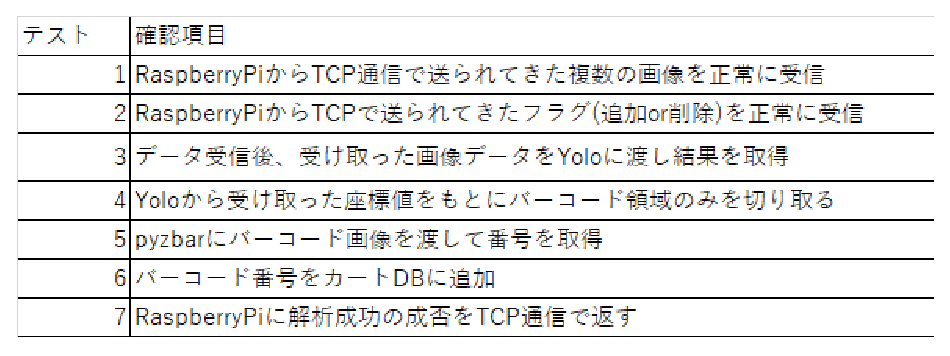
\includegraphics[width=15cm]{./pic/server_test.eps}
\label{server_test}
\end{table}

表\ref{yolo_test}は、メッセージ番号8のバーコード解析についての単体テスト項目である。
\begin{table}[htbp]
\centering
\caption{Yolo単体テスト項目}
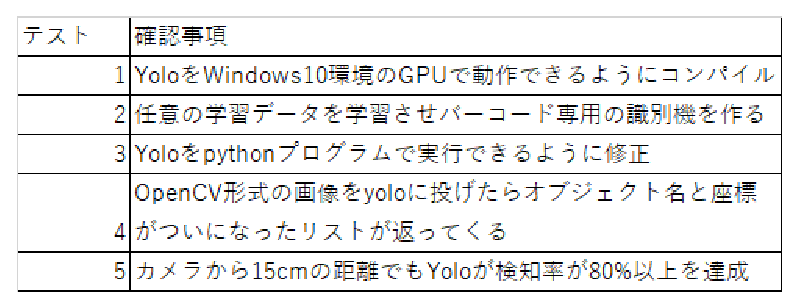
\includegraphics[width=15cm]{./pic/yolo_test.eps}
\label{yolo_test}
\end{table}

\newpage

表\ref{db_test}はメッセージ番号12~18の決済システムに対する単体テスト項目である。
\begin{table}[htbp]
\centering
\caption{決済システム単体テスト項目}
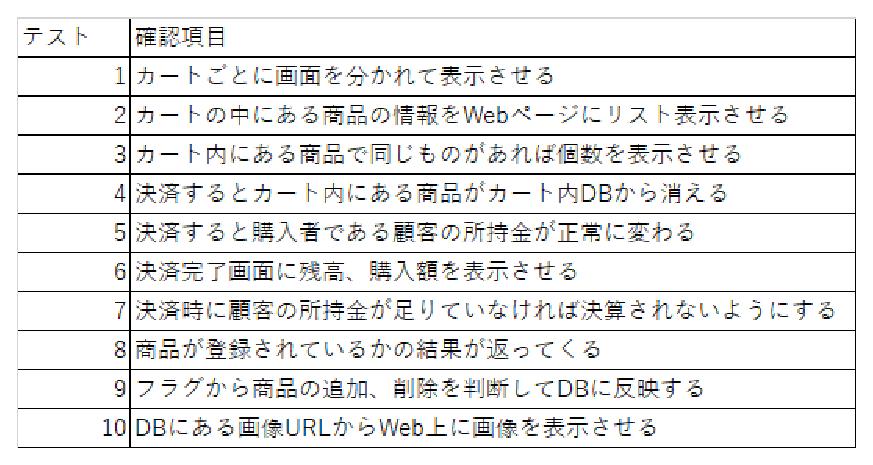
\includegraphics[width=15cm]{./pic/db_test.eps}
\label{db_test}
\end{table}

表\ref{server_test}は、メッセージ番号12の商品DBに対する単体テスト項目である。
\begin{table}[htbp]
\centering
\caption{商品DB単体テスト項目}
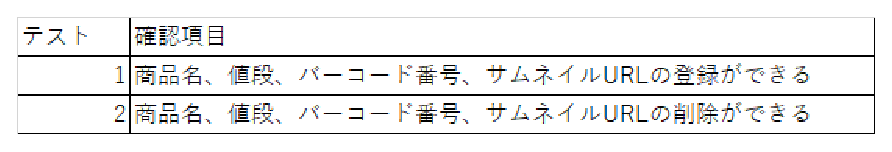
\includegraphics[width=15cm]{./pic/table_test.eps}
\label{table_test}
\end{table}
